\documentclass[11pt,letterpaper]{article}

% ============ DATOS DEL ESTUDIANTE ============
\newcommand{\nombreEstudiante}{Duván Felipe Baquero}
\newcommand{\codigoEstudiante}{160005002}
\newcommand{\nombreDocente}{Ángel Alfonso Cruz Roa}
% ==============================================

% Preámbulo agnóstico al motor: sirve con pdfLaTeX, XeLaTeX y LuaLaTeX.
\usepackage{iftex}
\ifPDFTeX
  \usepackage[utf8]{inputenc}
  \usepackage[T1]{fontenc}
  \usepackage{lmodern}
\else
  \usepackage{fontspec}
\fi

% babel-spanish redefine \% y rompe \,\% y el \% dentro de modo matemático.
\let\origpercent\%
\usepackage[spanish,es-tabla]{babel}
\AtBeginDocument{\let\%\origpercent}

\usepackage[margin=2.5cm]{geometry}
\usepackage{graphicx}
\usepackage{booktabs}
\usepackage{array}
\usepackage{amsmath}
\usepackage{amssymb}
\usepackage{float}
\usepackage{xcolor}
\usepackage{fancyhdr}
\usepackage{caption}
\usepackage{enumitem}
\usepackage{microtype}
\usepackage{tocloft}
\usepackage[hidelinks]{hyperref}

\setlength{\cftbeforesecskip}{0.7em}
\captionsetup{font=small,labelfont=bf,skip=6pt}
\setlength{\parskip}{0.35em}
\renewcommand{\arraystretch}{1.12}

\pagestyle{fancy}
\fancyhf{}
\lhead{\small Universidad de los Llanos}
\rhead{\small Simulación Computacional --- Práctica N.\textsuperscript{o}\,04}
\rfoot{\small\thepage}
\renewcommand{\headrulewidth}{0.4pt}

\begin{document}

% =====================================================
% PORTADA
% =====================================================
\begin{titlepage}
\thispagestyle{empty}
\centering
\vspace*{\fill}

{\large \textsc{Universidad de los Llanos}}\\[0.2cm]
{\normalsize Facultad de Ciencias Básicas e Ingeniería}\\
{\normalsize Programa de Ingeniería de Sistemas}\\[1.6cm]

\rule{\textwidth}{0.8pt}\\[0.5cm]
{\LARGE \textbf{Generación de variables\\ aleatorias continuas}}\\[0.35cm]
{\large Transformada inversa, rechazo, método polar\\
y procesos de Poisson homogéneos y no homogéneos}\\[0.5cm]
\rule{\textwidth}{0.8pt}\\[1.6cm]

{\normalsize Informe de la Práctica N.\textsuperscript{o}\,04}\\
{\normalsize Curso: Simulación Computacional}\\[1.4cm]

{\normalsize Presentado por:}\\[0.15cm]
{\large \nombreEstudiante}\\
{\normalsize Código: \codigoEstudiante}\\[1.2cm]

{\normalsize Docente:}\\[0.15cm]
{\large \nombreDocente}\\[1.6cm]

{\normalsize Villavicencio, Meta \\ \today}

\vspace*{\fill}
\end{titlepage}

\newpage
\tableofcontents
\newpage

% =====================================================
\section{Objetivos}
% =====================================================

Estos son los objetivos que trae la guía de laboratorio:

\begin{itemize}[itemsep=2pt]
    \item Generar secuencias de valores de una variable aleatoria de una distribución de probabilidad continua.
    \item Generar valores aleatorios de una distribución de probabilidad continua usando el método de la transformada inversa.
    \item Generar valores aleatorios de una distribución de probabilidad continua usando el método del rechazo.
    \item Generar valores aleatorios de una distribución de probabilidad continua usando el método polar para generar variables aleatorias normales.
    \item Generar valores aleatorios de una distribución de exponencial.
    \item Generar valores aleatorios de una distribución de probabilidad Gamma.
    \item Generar valores aleatorios de una distribución de probabilidad Normal estandar.
    \item Generar variables aleatorias de procesos de Poisson y procesos de Poisson no homogéneos.
\end{itemize}

% =====================================================
\section{Consulta previa}
% =====================================================

\subsection{¿Qué es una variable aleatoria?}

Es una función que asocia un número real a cada resultado de un experimento aleatorio. Con ella se
puede calcular con probabilidades usando números en vez de eventos. En esta práctica hay varias: el
tiempo que tarda un trabajador en terminar su tarea en el numeral 5.2 b), o la cantidad de eventos que
ocurren hasta el tiempo $T$ en un proceso de Poisson.

\subsection{¿Qué es una distribución de probabilidad?}

Es la forma en que la probabilidad total se reparte entre los valores posibles de la variable. Siempre
puede describirse con la función de distribución acumulada $F(x) = P\{X \le x\}$, que es no
decreciente y va de 0 a 1. En el caso discreto se usa además la función de masa
$p(x_i) = P\{X = x_i\}$, y en el continuo la función de densidad $f(x)$, que cumple
$P\{a \le X \le b\} = \int_a^b f(x)\,dx$.

\subsection{¿Cuál es la diferencia entre una distribución discreta y una continua?}

Una variable discreta toma valores aislados, en cantidad finita o numerable, y cada uno tiene su propia
probabilidad positiva; las probabilidades se suman. Una continua puede caer en cualquier punto de un
intervalo, la probabilidad de un valor exacto es cero y las probabilidades salen de integrar la
densidad. Eso también cambia la forma de generarlas. En el Laboratorio 2 la transformada inversa
consistía en buscar $U$ dentro de una tabla de probabilidades acumuladas; aquí se trata de despejar
$x$ de la ecuación $F(x) = U$.

\subsection{¿Cuál es la definición de la distribución exponencial?}

Una variable $X$ es exponencial con tasa $\lambda > 0$ si su densidad es
\[
f(x) = \lambda e^{-\lambda x}, \qquad x \ge 0,
\]
con acumulada $F(x) = 1 - e^{-\lambda x}$, media $1/\lambda$ y varianza $1/\lambda^2$. Es la única
distribución continua sin memoria, es decir, $P\{X > s + t \mid X > s\} = P\{X > t\}$, y por eso se
usa para modelar tiempos entre llegadas.

\subsection{¿Cuál es la definición de la distribución Gamma y sus parámetros?}

$X$ es Gamma con parámetros $(n, \lambda)$ si
\[
f(x) = \frac{\lambda e^{-\lambda x}(\lambda x)^{n-1}}{\Gamma(n)}, \qquad x \ge 0,
\]
donde $n > 0$ es el parámetro de forma, $\lambda > 0$ el de tasa y
$\Gamma(n) = \int_0^\infty e^{-y}y^{n-1}\,dy$. Su media es $n/\lambda$ y su varianza $n/\lambda^2$.
Si $n$ es entero, $X$ se distribuye igual que la suma de $n$ exponenciales independientes de tasa
$\lambda$. Con $n = 1$ se recupera la exponencial.

\subsection{¿Cuál es la definición de la distribución normal estándar y sus parámetros?}

Es la normal con media $\mu = 0$ y desviación estándar $\sigma = 1$:
\[
f(z) = \frac{1}{\sqrt{2\pi}}\,e^{-z^2/2}, \qquad -\infty < z < \infty.
\]
Cualquier $N(\mu, \sigma^2)$ se obtiene de ella haciendo $X = \mu + \sigma Z$. Su acumulada no tiene
forma cerrada, así que no se puede invertir directamente y hay que usar el rechazo o el método polar.

\subsection{¿Qué es un proceso de Poisson y uno no homogéneo? ¿En qué se diferencian?}

Un proceso de Poisson de tasa $\lambda$ es un proceso de conteo $\{N(t), t \ge 0\}$ con $N(0) = 0$,
incrementos independientes y estacionarios, y en el que el número de eventos en cualquier intervalo de
longitud $t$ es Poisson de media $\lambda t$. De ahí se deduce que los tiempos entre eventos son
exponenciales independientes de tasa $\lambda$.

En el no homogéneo la tasa depende del tiempo a través de una función de intensidad $\lambda(t)$. Los
incrementos siguen siendo independientes pero dejan de ser estacionarios, y el número de eventos entre
$s$ y $s+t$ es Poisson de media $\int_s^{s+t}\lambda(y)\,dy$. En pocas palabras, en el homogéneo da
igual en qué momento se observe una ventana de tiempo de cierto largo, y en el no homogéneo no: no
llega la misma cantidad de clientes a un restaurante a las siete de la mañana que al mediodía. Como los
tiempos entre eventos ya no son exponenciales idénticos, hace falta otro algoritmo para generarlo, como
el de adelgazamiento.

% =====================================================
\section{Metodología y herramientas}
% =====================================================

Todo el desarrollo está en un único cuaderno de Jupyter en Python, ejecutado de principio a fin:

\begin{center}
\texttt{Lab4\_\codigoEstudiante.ipynb}
\end{center}

Usa solamente \texttt{numpy}, \texttt{pandas}, \texttt{matplotlib} y \texttt{scipy}, que vienen
instalados en Google Colab. Los algoritmos de generación (transformada inversa, rechazo, polar,
Gamma, procesos de Poisson y adelgazamiento) están escritos a mano siguiendo el capítulo 5 de
\cite{ross99}. De \texttt{scipy} solo se toman las densidades y acumuladas teóricas para comparar, la
prueba de Kolmogorov--Smirnov, una integración numérica para las medias y varianzas teóricas y la
exponencial de matrices para la densidad de Coxian.

\subsection{Generador de números pseudoaleatorios}

La guía pide usar generadores congruenciales mixtos que cumplan los criterios de uniformidad y
aleatoriedad. Se tomó
\[
X_{n+1} = (a X_n + c) \bmod m, \qquad U_n = X_n/m,
\]
con $a = 25214903917$, $c = 11$ y $m = 2^{48}$, que en el Laboratorio 2 fue el único de los doce
generadores estudiados que pasó todas las pruebas con periodo completo. Cumple las tres condiciones de
Hull--Dobell: $\gcd(11, 2^{48}) = 1$, el único primo que divide a $m$ es 2 y divide a $a - 1$, y como
$4 \mid m$ también $4 \mid (a-1)$. Su periodo es entonces $2^{48} \approx 2{,}8\times10^{14}$, mucho
más de lo que consume cualquier parte de esta práctica.

Antes de usarlo se probaron 10\,000 valores con semilla 20260925. La tabla \ref{tab:gcm} muestra que
pasa las tres pruebas con holgura.

\begin{table}[H]
\centering
\caption{Pruebas sobre 10\,000 valores del generador congruencial mixto ($\alpha = 0{,}05$).}
\label{tab:gcm}
\small
\begin{tabular}{@{}lrrl@{}}
\toprule
Prueba & Estadístico & Valor $p$ & Decisión \\
\midrule
Kolmogorov--Smirnov (uniformidad)      & $D = 0{,}0071$      & 0,696 & No se rechaza $H_0$ \\
$\chi^2$ con 20 clases (uniformidad)   & $\chi^2 = 11{,}84$  & 0,892 & No se rechaza $H_0$ \\
Rachas arriba y abajo (aleatoriedad)   & $Z = 0{,}917$       & 0,359 & No se rechaza $H_0$ \\
\bottomrule
\end{tabular}
\end{table}

La media muestral dio 0,4977 y la varianza 0,0838, frente a los valores teóricos 0,5 y 0,0833. En el
cuaderno cada literal crea su propia instancia del generador con una semilla distinta, para que los
resultados de un literal no dependan de cuántos números gastó el anterior. Como las semillas están
fijas, cualquier ejecución reproduce exactamente las cifras de este informe.

\subsection{Criterio de validación}

En cada caso se generaron 1000 valores, se dibujó su histograma normalizado como densidad y encima la
densidad teórica como línea continua, que es lo que pide la guía. Además de la comparación visual se
calcularon la media y la varianza muestrales frente a las teóricas y se aplicó la prueba de
Kolmogorov--Smirnov contra la acumulada teórica. Un valor $p$ mayor que 0,05 indica que no hay
evidencia para decir que la muestra no viene de la distribución buscada.

\subsection{Generadores de apoyo: exponencial, Gamma y normal estándar}

Tres de los objetivos piden generar exponenciales, Gamma y normales estándar, aunque el procedimiento no
los trae como literales. Se implementaron al comienzo porque la exponencial se necesita después en los
procesos de Poisson y en la variable de Coxian:

\begin{itemize}[itemsep=2pt]
\item Exponencial por transformada inversa: $X = -\frac{1}{\lambda}\ln U$.
\item Gamma$(n, \lambda)$ con $n$ entero: $X = -\frac{1}{\lambda}\ln(U_1 U_2\cdots U_n)$, que equivale a
sumar $n$ exponenciales pero con un solo logaritmo.
\item Normal estándar por el método polar: se generan $V_1, V_2 \sim U(-1,1)$ hasta que
$S = V_1^2 + V_2^2 \le 1$ y se devuelven $V_1\sqrt{-2\ln S/S}$ y $V_2\sqrt{-2\ln S/S}$.
\end{itemize}

\begin{figure}[H]
\centering
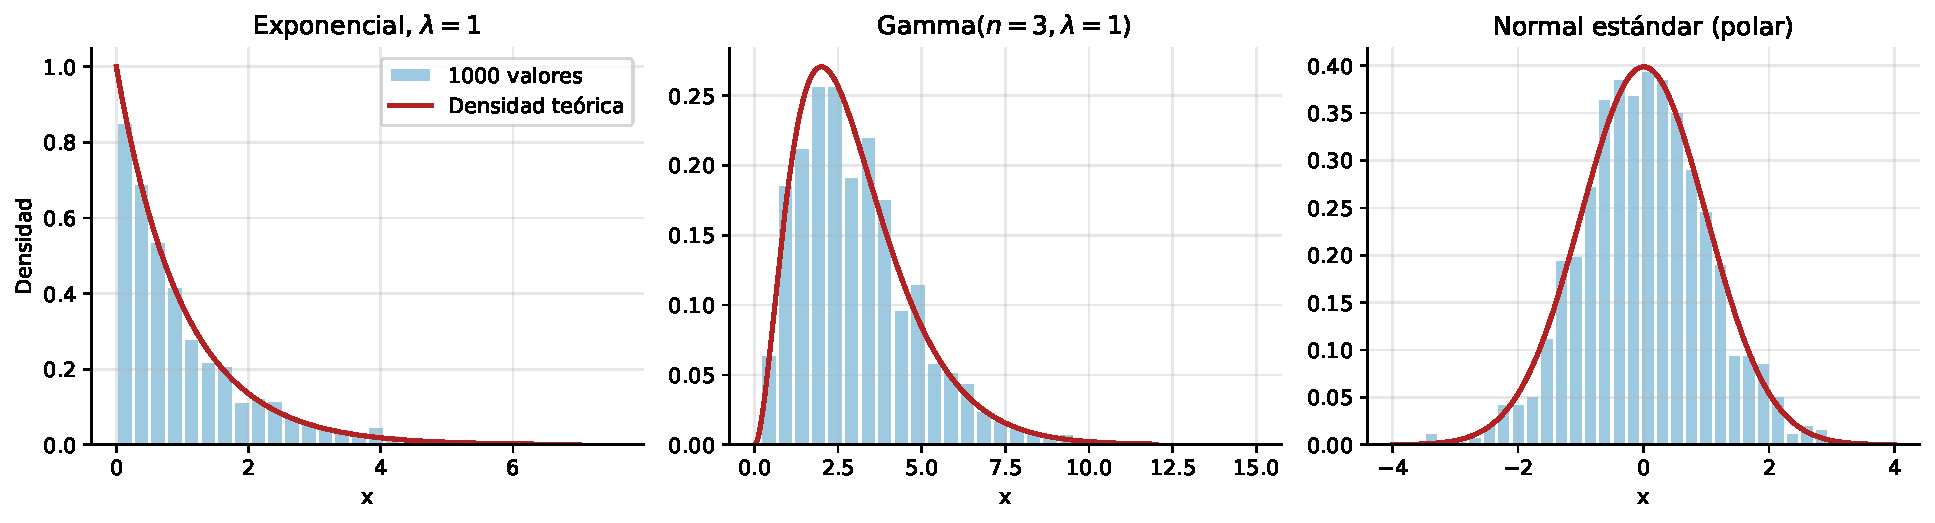
\includegraphics[width=\textwidth]{fig_apoyo.pdf}
\caption{Exponencial$(1)$, Gamma$(3, 1)$ y normal estándar por el método polar, 1000 valores cada una.}
\label{fig:apoyo}
\end{figure}

\begin{table}[H]
\centering
\caption{Resumen de los generadores de apoyo.}
\label{tab:apoyo}
\small
\begin{tabular}{@{}lrrrrrr@{}}
\toprule
Distribución & Media sim. & Media teór. & Var. sim. & Var. teór. & $D$ (KS) & Valor $p$ \\
\midrule
Exponencial$(1)$ & 1,0525 & 1 & 1,1401 & 1 & 0,0281 & 0,402 \\
Gamma$(3, 1)$    & 3,0796 & 3 & 3,3469 & 3 & 0,0338 & 0,199 \\
Normal$(0, 1)$   & 0,0096 & 0 & 1,0313 & 1 & 0,0203 & 0,797 \\
\bottomrule
\end{tabular}
\end{table}

Ninguna de las tres se rechaza. En el método polar se necesitaron 628 intentos para obtener 500 pares,
una tasa de aceptación de 0,796. La teórica es $\pi/4 \approx 0{,}785$, la fracción del cuadrado
$[-1,1]^2$ que ocupa el círculo unitario.

% =====================================================
\section{Numeral 5.1: generación de variables aleatorias continuas}
% =====================================================

\subsection{Literal a): $f(x) = e^x/(e-1)$ en $[0, 1]$}

La acumulada se obtiene integrando directamente:
\[
F(x) = \int_0^x \frac{e^y}{e-1}\,dy = \frac{e^x - 1}{e - 1}, \qquad 0 \le x \le 1.
\]
Al igualarla a $U$ queda $e^x = 1 + (e-1)U$, y por \textbf{transformada inversa}
\[
X = \ln\big(1 + (e-1)U\big).
\]

\begin{figure}[H]
\centering
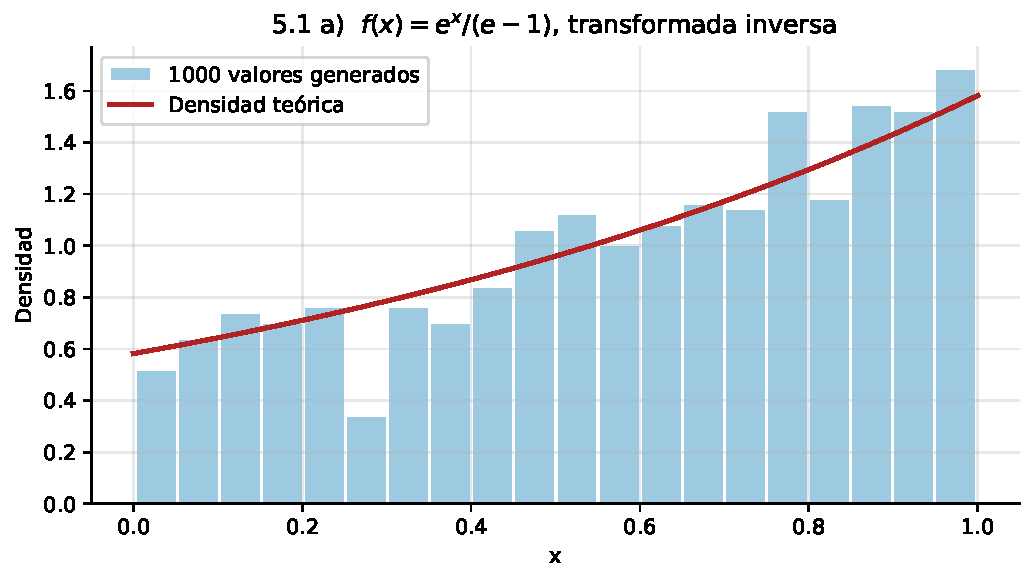
\includegraphics[width=0.72\textwidth]{fig_51a.pdf}
\caption{Literal a): histograma de los 1000 valores y densidad teórica.}
\label{fig:51a}
\end{figure}

La barra baja cerca de $x = 0{,}3$ llama la atención, pero es variación de muestreo normal con 20
clases de 50 valores esperados en promedio; la prueba de Kolmogorov--Smirnov, que no depende de cómo se
agrupen los datos, da $p = 0{,}162$. La media simulada fue 0,5963 frente a
$1/(e-1) = 0{,}5820$.

\subsection{Literal b): densidad triangular en $[2, 6]$}

La densidad
\[
f(x) = \begin{cases} \dfrac{x-2}{2}, & 2 \le x \le 3,\\[2mm] \dfrac{2 - x/3}{2}, & 3 \le x \le 6,\end{cases}
\]
es una triangular con mínimo 2, moda 3 y máximo 6, y su valor más alto es $f(3) = 1/2$. Este literal
se resolvió con el \textbf{método del rechazo}, que es el que piden los objetivos, y también con la
inversa para comparar.

\textbf{Rechazo.} Como el soporte es finito y la densidad está acotada, sirve como auxiliar la uniforme
en $[2, 6]$, con $g(y) = 1/4$. La constante es $c = \max f/g = (1/2)/(1/4) = 2$ y la regla de
aceptación queda $U \le f(Y)/(c\,g(Y)) = 2f(Y)$.

\textbf{Inversa.} Integrando por tramos,
\[
F(x) = \begin{cases} \dfrac{(x-2)^2}{4}, & 2 \le x \le 3,\\[2mm] x - \dfrac{x^2}{12} - 2, & 3 \le x \le 6,\end{cases}
\]
con $F(3) = 1/4$. Despejando: $X = 2 + 2\sqrt{U}$ si $U \le 1/4$, y $X = 6 - 2\sqrt{3(1-U)}$ si
$U > 1/4$.

\begin{figure}[H]
\centering
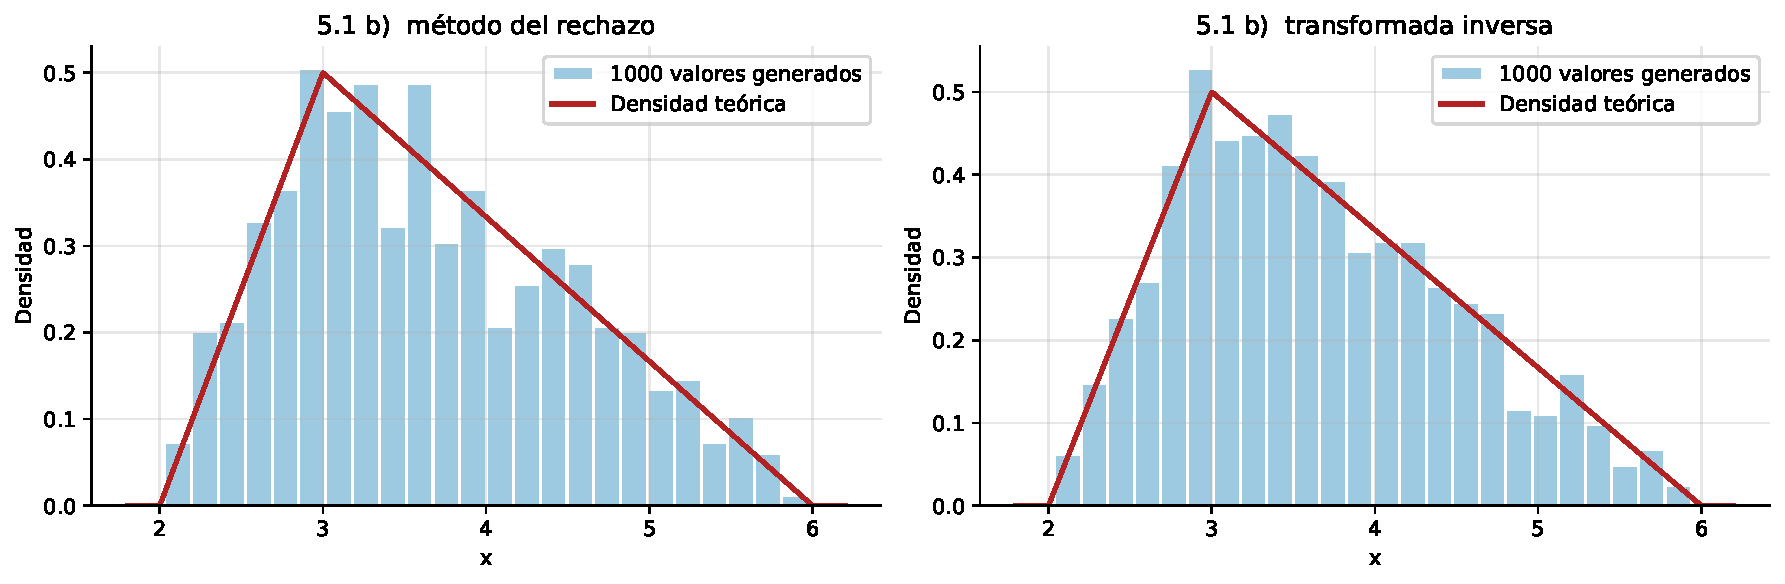
\includegraphics[width=\textwidth]{fig_51b.pdf}
\caption{Literal b): método del rechazo (izquierda) y transformada inversa (derecha).}
\label{fig:51b}
\end{figure}

Los dos métodos dan la misma forma triangular. El rechazo necesitó en promedio 1,988 iteraciones por
valor aceptado, casi exactamente las $c = 2$ que predice la teoría, y como cada iteración gasta dos
uniformes terminó consumiendo 3976 números, contra 1000 de la inversa. En este caso la inversa es la
mejor opción porque la acumulada se deja despejar. El rechazo vale la pena cuando eso no pasa, como con
la normal.

\subsection{Literal c): $F(x) = (x^2 + x)/2$ en $[0, 1]$}

La guía pide transformada inversa. De $F(x) = U$ sale la cuadrática $x^2 + x - 2U = 0$, y la raíz que
cae en $[0,1]$ es
\[
X = \frac{-1 + \sqrt{1 + 8U}}{2}.
\]
La densidad que se dibuja encima es $f(x) = F'(x) = x + \tfrac{1}{2}$.

\begin{figure}[H]
\centering
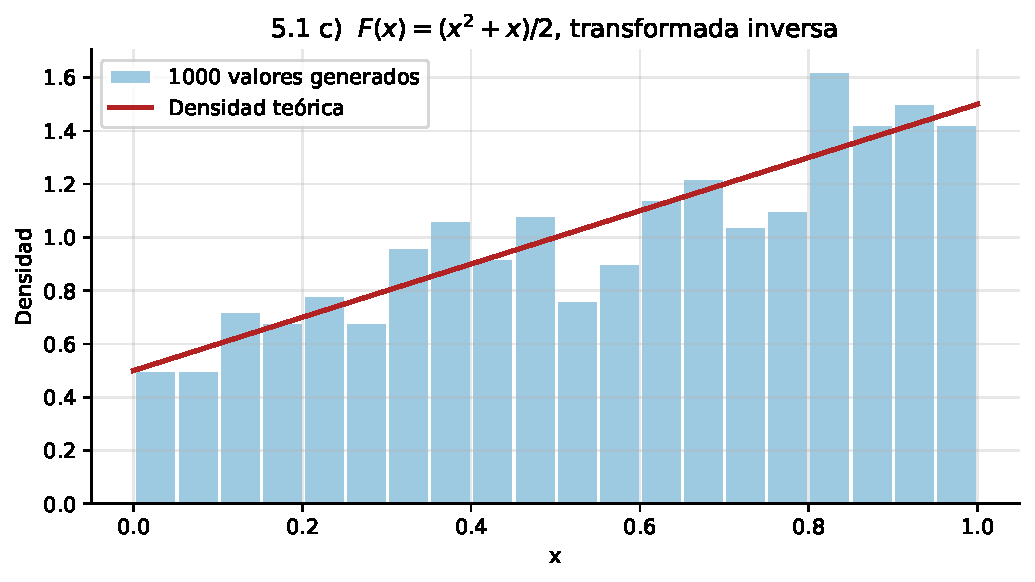
\includegraphics[width=0.72\textwidth]{fig_51c.pdf}
\caption{Literal c): histograma de los 1000 valores y densidad teórica $f(x) = x + 1/2$.}
\label{fig:51c}
\end{figure}

\subsection{Literal d): distribución de Weibull}

De $1 - e^{-\alpha x^\beta} = U$ se despeja $X = \left(-\frac{1}{\alpha}\ln(1-U)\right)^{1/\beta}$.
Como $1 - U$ también es uniforme en $(0,1)$ se usa
\[
X = \left(-\frac{\ln U}{\alpha}\right)^{1/\beta},
\]
que ahorra una resta. La densidad es $f(x) = \alpha\beta x^{\beta-1}e^{-\alpha x^\beta}$ y la media
$E[X] = \alpha^{-1/\beta}\,\Gamma(1 + 1/\beta)$. La guía no da valores para $\alpha$ y $\beta$, así que
se probaron tres combinaciones con formas bien distintas: $\beta = 1$, donde la Weibull se reduce a la
exponencial de tasa $\alpha$; $\beta = 2$, que es la Rayleigh; y $\beta = 3{,}5$ con $\alpha = 0{,}5$,
que queda casi simétrica.

\begin{figure}[H]
\centering
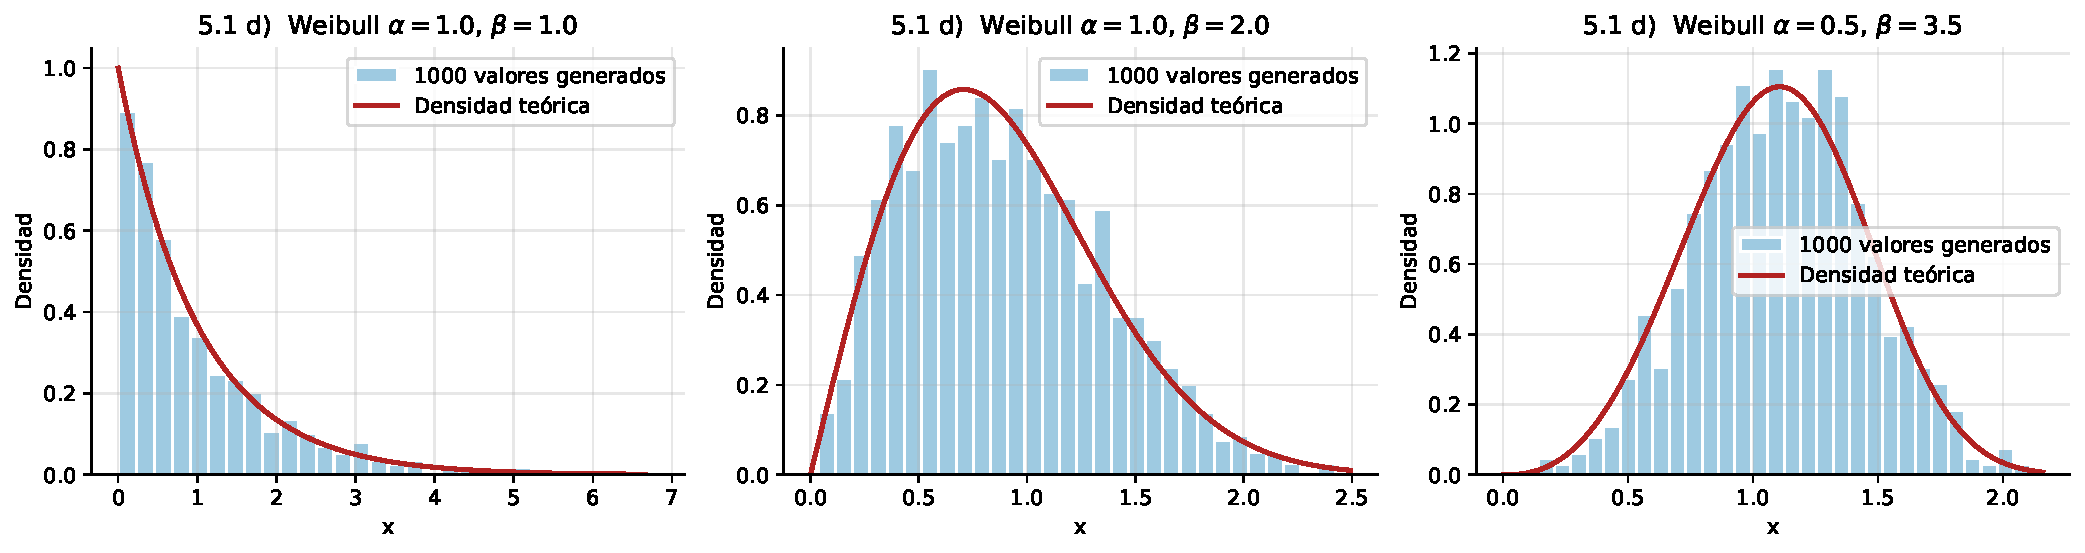
\includegraphics[width=\textwidth]{fig_51d.pdf}
\caption{Literal d): Weibull con tres pares de parámetros, 1000 valores cada uno.}
\label{fig:51d}
\end{figure}

\subsection{Resumen del numeral}

\begin{table}[H]
\centering
\caption{Momentos y prueba de Kolmogorov--Smirnov para los 1000 valores de cada caso.}
\label{tab:51}
\small\setlength{\tabcolsep}{5pt}
\begin{tabular}{@{}lrrrrrrr@{}}
\toprule
Caso & Media sim. & Media teór. & Error & Var. sim. & Var. teór. & $D$ & Valor $p$ \\
\midrule
a) $e^x/(e-1)$                        & 0,5963 & 0,5820 & 2,46\,\% & 0,0778 & 0,0793 & 0,0353 & 0,162 \\
b) triangular, rechazo                & 3,6541 & 3,6667 & 0,34\,\% & 0,7715 & 0,7222 & 0,0271 & 0,447 \\
b) triangular, inversa                & 3,6428 & 3,6667 & 0,65\,\% & 0,7086 & 0,7222 & 0,0206 & 0,780 \\
c) $(x^2+x)/2$                        & 0,5827 & 0,5833 & 0,10\,\% & 0,0771 & 0,0764 & 0,0204 & 0,790 \\
d) Weibull $\alpha = 1$, $\beta = 1$     & 1,0186 & 1,0000 & 1,86\,\% & 1,0934 & 1,0000 & 0,0248 & 0,561 \\
d) Weibull $\alpha = 1$, $\beta = 2$     & 0,8909 & 0,8862 & 0,52\,\% & 0,2084 & 0,2146 & 0,0189 & 0,859 \\
d) Weibull $\alpha = 0{,}5$, $\beta = 3{,}5$ & 1,1157 & 1,0968 & 1,72\,\% & 0,1149 & 0,1205 & 0,0308 & 0,291 \\
\bottomrule
\end{tabular}
\end{table}

Todos los valores $p$ superan 0,05 y el error en la media nunca pasa de 2,5\,\%. Con 1000 datos el
error estándar de la media es $\sigma/\sqrt{1000} \approx 3{,}2\,\%$ de $\sigma$, así que diferencias
de ese tamaño son las esperables. Por ejemplo, en el literal a) la media se desvió 0,0143, que
equivale a 1,6 errores estándar ($\sigma = 0{,}282$).

% =====================================================
\section{Numeral 5.2: generando procesos de Poisson}
% =====================================================

\subsection{Literal a): primeras $T$ unidades de tiempo de un proceso de Poisson}

Se programó el algoritmo de la sección 5.4 de \cite{ross99}, que genera los tiempos entre eventos como
exponenciales y los va acumulando:

\begin{enumerate}[itemsep=1pt,label=\textsc{Paso} \arabic*:,leftmargin=5em]
\item $t = 0$, $I = 0$.
\item Generar $U$.
\item $t = t - \frac{1}{\lambda}\ln U$. Si $t > T$, parar.
\item $I = I + 1$, $S(I) = t$.
\item Volver al paso 2.
\end{enumerate}

Al terminar, $I = N(T)$ y $S(1), \dots, S(I)$ son los tiempos de los eventos. La función recibe
$\lambda$ y $T$ como parámetros; para mostrarla se usó $\lambda = 2$ y $T = 10$. La realización de la
figura \ref{fig:52a} tuvo 18 eventos, dos menos de los 20 esperados.

\begin{figure}[H]
\centering
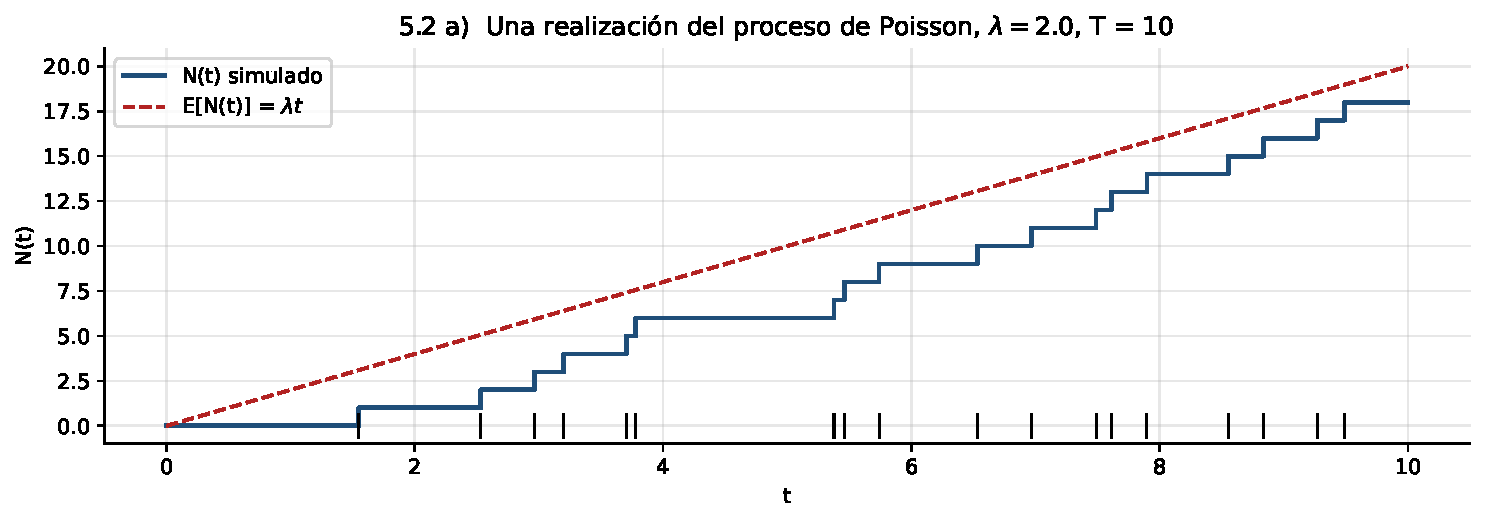
\includegraphics[width=0.85\textwidth]{fig_52a_realizacion.pdf}
\caption{Una realización del proceso con $\lambda = 2$ y $T = 10$. Las marcas sobre el eje son los
tiempos de los eventos.}
\label{fig:52a}
\end{figure}

Para verificar el programa se repitió 1000 veces y se revisaron tres propiedades. $N(10)$ dio media
19,955 y varianza 18,642, las dos cerca de 20, como corresponde a una Poisson de media
$\lambda T = 20$. El primer tiempo entre eventos $S(1)$ tuvo media 0,5167 y pasó la prueba contra la
exponencial de tasa 2 ($D = 0{,}0240$, $p = 0{,}602$). Por último, los 19\,955 tiempos de ocurrencia
juntos pasaron la prueba de uniformidad en $[0, 10]$ con $p = 0{,}794$, lo que concuerda con que,
dado $N(T)$, los tiempos de los eventos se reparten de manera uniforme en el intervalo.

\begin{figure}[H]
\centering
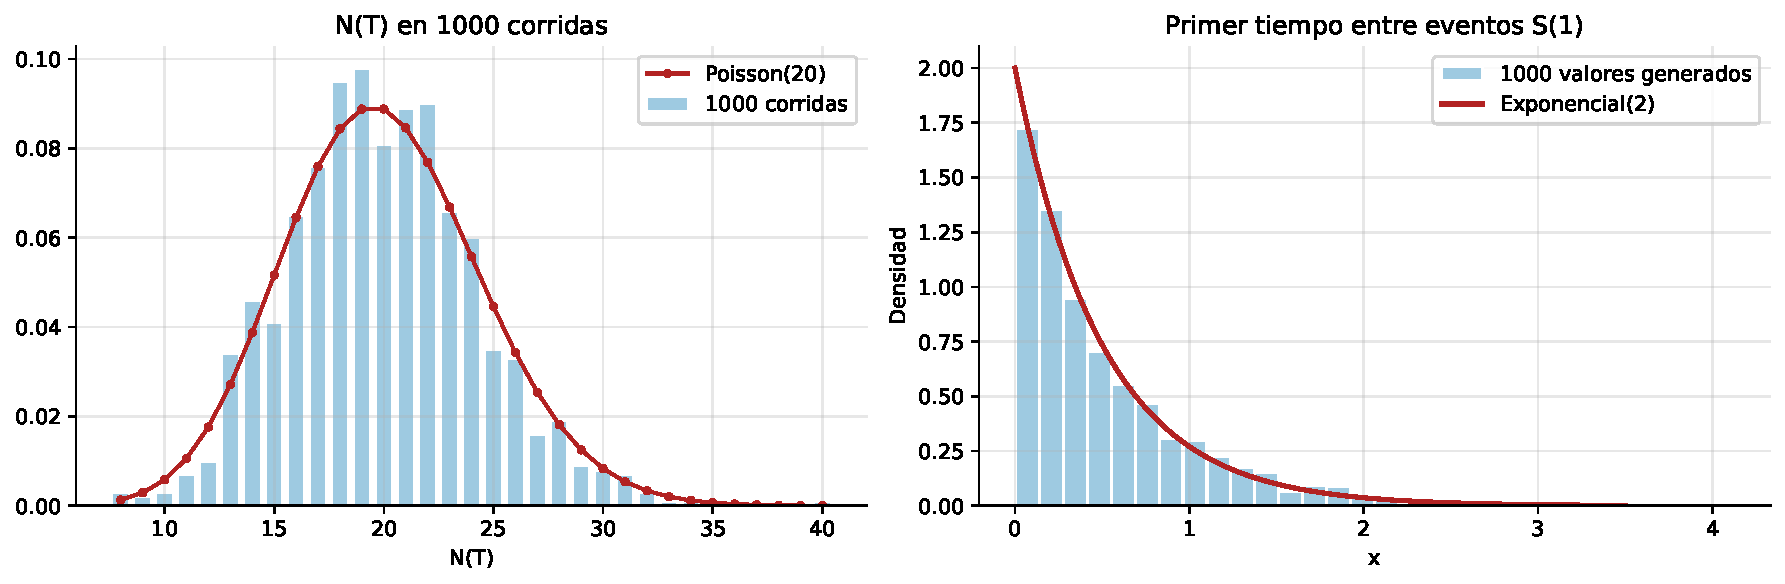
\includegraphics[width=\textwidth]{fig_52a_validacion.pdf}
\caption{Distribución de $N(10)$ contra Poisson(20) y del primer tiempo entre eventos contra
Exponencial(2), en 1000 corridas.}
\label{fig:52aval}
\end{figure}

Hubo un detalle en la validación que vale la pena contar. La primera idea fue juntar todos los tiempos
entre eventos de las 1000 corridas y compararlos con la exponencial, y la prueba de
Kolmogorov--Smirnov los rechazó ($p < 0{,}0001$) con una media de 0,4778 en lugar de 0,5. El generador
no estaba mal. Al cortar cada corrida en $T = 10$ se descarta el último intervalo, el que no alcanzó a
cerrarse, y los intervalos largos tienen más probabilidad de ser ese último. La muestra queda así
sesgada hacia valores pequeños. Una cuenta rápida lo confirma: la suma de los intervalos observados es
$S(N)$, que en promedio vale cerca de $10 - 0{,}5 = 9{,}5$, y dividida entre 20 eventos da 0,475,
prácticamente lo que se midió. Por eso la comparación se hizo con $S(1)$, que casi nunca queda cortado
($P\{S(1) > 10\} = e^{-20}$).

\subsection{Literal b): variable aleatoria de Coxian}

El trabajador recorre las etapas $1, \dots, k$ en orden. La etapa $i$ dura una exponencial de tasa
$\lambda_i$ y al terminarla sigue a la siguiente con probabilidad $\alpha_i$ o se retira con
probabilidad $1 - \alpha_i$. $X$ es el tiempo total. Después de la etapa $k$ el trabajo termina de
todas formas, así que $\alpha_k$ no se usa. El algoritmo propuesto es:

\begin{enumerate}[itemsep=1pt,label=\textsc{Paso} \arabic*:,leftmargin=5em]
\item $X = 0$, $i = 1$.
\item Generar $U_1$ y hacer $X = X - \frac{1}{\lambda_i}\ln U_1$.
\item Si $i = k$, devolver $X$.
\item Generar $U_2$. Si $U_2 > \alpha_i$, devolver $X$.
\item $i = i + 1$ y volver al paso 2.
\end{enumerate}

Para probarlo se tomó $k = 3$, $\lambda = (1;\ 2;\ 0{,}5)$ y $\alpha = (0{,}7;\ 0{,}4)$ y se generaron
1000 valores. Hay tres cosas contra las cuales comparar. La probabilidad de retirarse justo en la etapa
$i$ es $\alpha_1\cdots\alpha_{i-1}(1 - \alpha_i)$, que da 0,30, 0,42 y 0,28. La media es
\[
E[X] = \sum_{i=1}^{k}\frac{\alpha_1\cdots\alpha_{i-1}}{\lambda_i} = \frac{1}{1} + \frac{0{,}7}{2} + \frac{0{,}28}{0{,}5} = 1{,}91.
\]
Y la densidad exacta se puede escribir porque la Coxian es una distribución tipo fase: con
$\mathbf{a} = (1, 0, 0)$ y la matriz $\mathbf{S}$ que tiene $-\lambda_i$ en la diagonal y
$\alpha_i\lambda_i$ justo encima,
\[
f(x) = \mathbf{a}\,e^{\mathbf{S}x}\,\mathbf{s}_0, \qquad \mathbf{s}_0 = -\mathbf{S}\mathbf{1}.
\]

\begin{table}[H]
\centering
\caption{Etapa en la que termina el trabajo, 1000 valores simulados.}
\label{tab:coxian}
\small
\begin{tabular}{@{}crr@{}}
\toprule
Etapa final & Frecuencia simulada & Probabilidad teórica \\
\midrule
1 & 0,300 & 0,30 \\
2 & 0,419 & 0,42 \\
3 & 0,281 & 0,28 \\
\bottomrule
\end{tabular}
\end{table}

\begin{figure}[H]
\centering
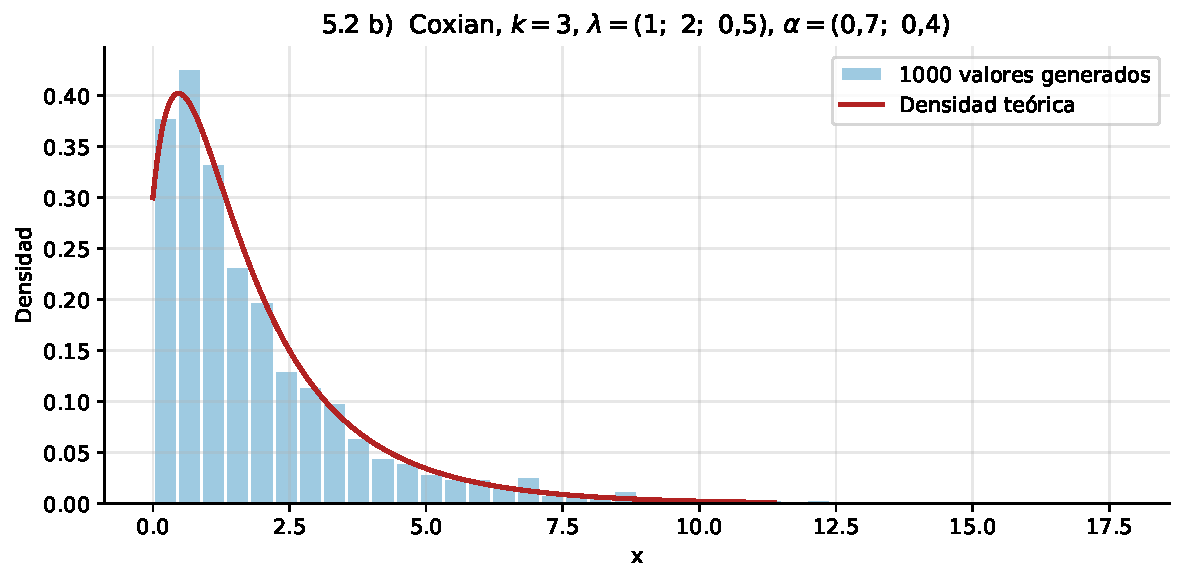
\includegraphics[width=0.75\textwidth]{fig_52b_coxian.pdf}
\caption{Variable de Coxian: histograma de 1000 valores y densidad tipo fase exacta.}
\label{fig:coxian}
\end{figure}

Las frecuencias por etapa coinciden con las teóricas casi al tercer decimal. La media simulada dio
1,9736 frente a 1,91 y la prueba de Kolmogorov--Smirnov contra la acumulada exacta no rechaza
($D = 0{,}0306$, $p = 0{,}302$). La forma de la densidad es interesante: arranca en
$f(0) = \lambda_1(1 - \alpha_1) = 0{,}3$ y no en 1, como haría una exponencial de tasa 1, porque en
$x = 0$ solo contribuye quien se retira en la primera etapa. Además tiene una cola larga que viene de
la tercera etapa, la más lenta, con media 2.

% =====================================================
\section{Numeral 5.3: proceso de Poisson no homogéneo}
% =====================================================

\subsection{Planteamiento}

La función de intensidad es
\[
\lambda(t) = \begin{cases} \dfrac{t}{5}, & 0 < t < 5,\\[2mm] 1 + 5(t - 5), & 5 < t < 10.\end{cases}
\]
Las dos ramas valen 1 en $t = 5$, así que es continua y creciente, con máximo $\lambda(10) = 26$. El
número esperado de eventos en $[0, 10]$ es
\[
m(10) = \int_0^5 \frac{t}{5}\,dt + \int_5^{10}\big(1 + 5(t - 5)\big)\,dt = 2{,}5 + 67{,}5 = 70.
\]
Casi todo ocurre en la segunda mitad: se esperan 2,5 eventos antes de $t = 5$ y 67,5 después.

\subsection{Algoritmo de adelgazamiento}

Se implementó el algoritmo de la sección 5.5 de \cite{ross99} con la cota $\lambda = 26$:

\begin{enumerate}[itemsep=1pt,label=\textsc{Paso} \arabic*:,leftmargin=5em]
\item $t = 0$, $I = 0$.
\item Generar $U$.
\item $t = t - \frac{1}{\lambda}\ln U$. Si $t > T$, parar.
\item Generar $U$.
\item Si $U \le \lambda(t)/\lambda$, hacer $I = I + 1$ y $S(I) = t$.
\item Volver al paso 2.
\end{enumerate}

La idea es generar un proceso homogéneo de tasa 26 y quedarse con cada evento con probabilidad
$\lambda(t)/26$. En la realización de la figura \ref{fig:53} se generaron 252 candidatos y se
aceptaron 69: 4 en $(0, 5]$ y 65 en $(5, 10]$.

\begin{figure}[H]
\centering
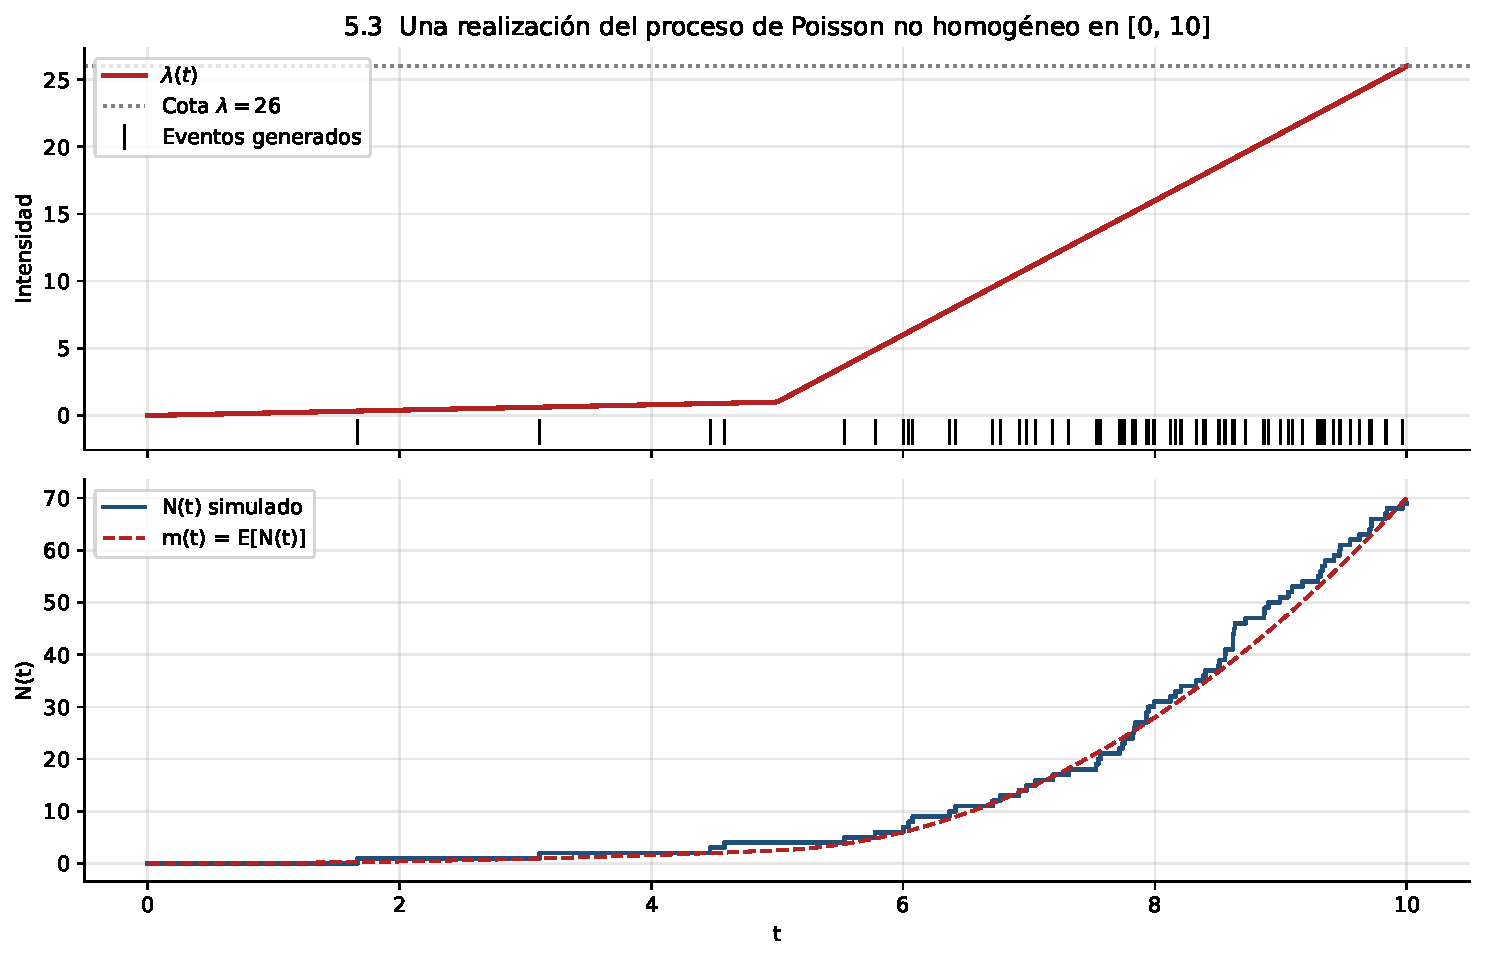
\includegraphics[width=0.9\textwidth]{fig_53_realizacion.pdf}
\caption{Arriba, la intensidad $\lambda(t)$, la cota $\lambda = 26$ y los 69 eventos generados. Abajo,
el conteo $N(t)$ contra su valor esperado $m(t)$.}
\label{fig:53}
\end{figure}

\subsection{Versión por subintervalos}

Con una sola cota se desperdicia mucho trabajo en $[0, 5]$, donde $\lambda(t) \le 1$ y casi todos los
candidatos se rechazan. En la misma sección 5.5 Ross propone partir el intervalo y usar una cota para
cada parte, reaprovechando la exponencial que se sale de un subintervalo mediante el reescalamiento
$X \leftarrow (X - t_j + t)\lambda_j/\lambda_{j+1}$. Aquí el corte natural es $t = 5$, con
$\lambda_1 = 1$ en $[0, 5]$ y $\lambda_2 = 26$ en $[5, 10]$. Esa versión también quedó implementada
en el cuaderno.

\subsection{Resultados de 1000 corridas}

\begin{table}[H]
\centering
\caption{Comparación de los dos algoritmos en 1000 corridas.}
\label{tab:53}
\small\setlength{\tabcolsep}{5pt}
\begin{tabular}{@{}lrrrrrr@{}}
\toprule
Algoritmo & Media $N(10)$ & Var. $N(10)$ & \multicolumn{2}{c}{Candidatos} & Aceptación & $p$ (KS) \\
\cmidrule(lr){4-5}
 & & & sim. & teór. & & \\
\midrule
Adelgazamiento, $\lambda = 26$        & 69,998 & 68,40 & 260,05 & 260 & 26,9\,\% & 0,411 \\
Por subintervalos, $\lambda = (1;\ 26)$ & 70,355 & 73,27 & 135,29 & 135 & 52,0\,\% & 0,152 \\
\bottomrule
\end{tabular}
\begin{minipage}{0.92\textwidth}\vspace{2pt}\footnotesize
La columna KS compara todos los tiempos de los eventos juntos contra la densidad $\lambda(t)/70$ en
$[0, 10]$, cuya acumulada es $m(t)/70$.
\end{minipage}
\end{table}

\begin{figure}[H]
\centering
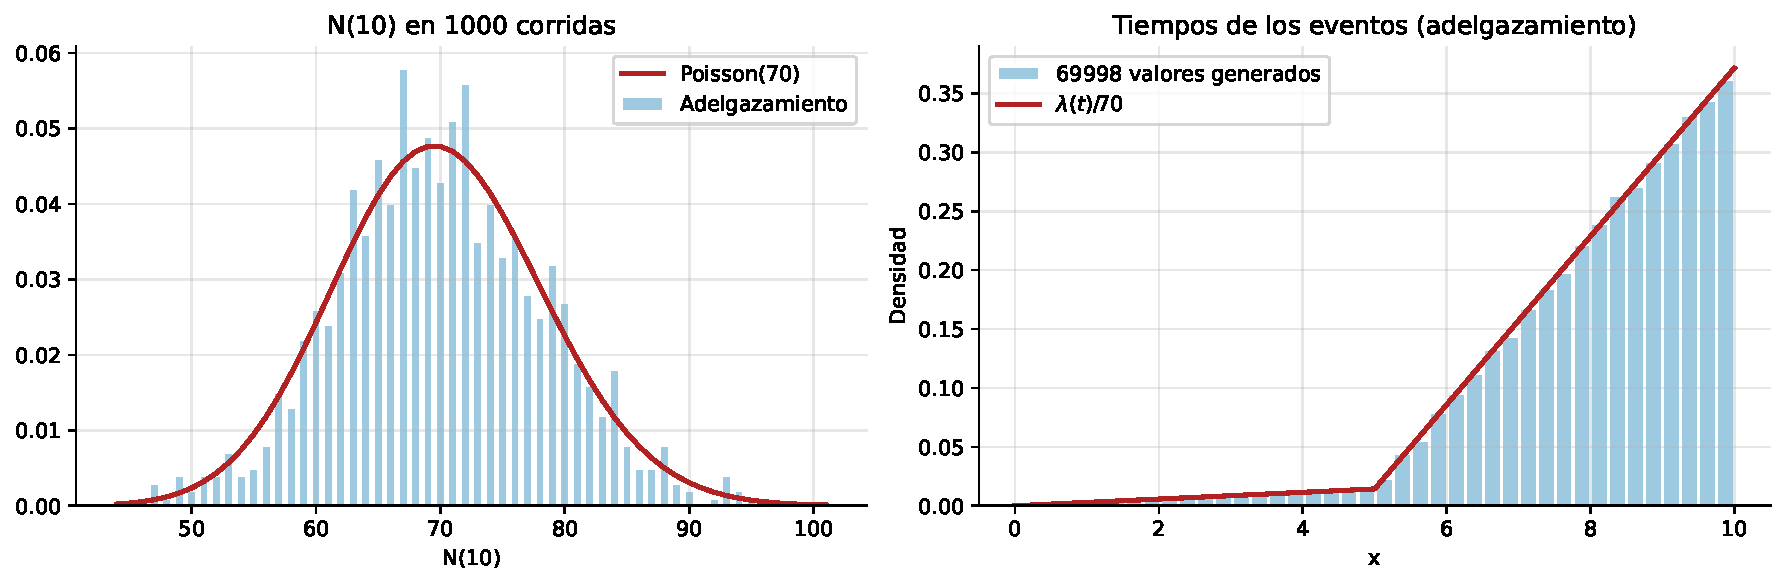
\includegraphics[width=\textwidth]{fig_53_validacion.pdf}
\caption{Izquierda, $N(10)$ en 1000 corridas contra Poisson(70). Derecha, los tiempos de todos los
eventos contra la densidad $\lambda(t)/70$.}
\label{fig:53val}
\end{figure}

Los dos algoritmos generan el mismo proceso. La media y la varianza de $N(10)$ quedan alrededor de 70,
como debe ser en una Poisson de media 70, y el histograma de los tiempos sigue la forma de $\lambda(t)$:
casi plano y bajo hasta $t = 5$ y luego una rampa. La diferencia está en el costo. Con una sola cota se
generaron en promedio 260 candidatos por corrida y se aceptó el 26,9\,\%. Con el corte en $t = 5$ los
candidatos bajaron a 135 y la aceptación subió a 52\,\%, es decir, la mitad de trabajo para el mismo
resultado. Todavía se podría mejorar partiendo $[5, 10]$ en tramos más cortos, porque ahí la intensidad
sube de 1 a 26 y la cota fija sigue rechazando cerca de la mitad.

% =====================================================
\section{Conclusiones}
% =====================================================

\begin{enumerate}[itemsep=4pt]

\item Cuando la acumulada se puede despejar, la transformada inversa es el método más directo y el
más barato: un número uniforme por valor. Así se resolvieron los literales a), c) y d) del numeral 5.1,
y las siete muestras de ese numeral pasaron la prueba de Kolmogorov--Smirnov con valores $p$ entre
0,16 y 0,86.

\item El rechazo funcionó tal como lo predice la teoría. En la triangular del literal b) necesitó
1,988 iteraciones por valor frente a $c = 2$, y el polar aceptó el 79,6\,\% de los pares frente a
$\pi/4 = 78{,}5\,\%$. Pero cuesta: en el literal b) gastó unas cuatro veces más números uniformes que
la inversa. Su lugar está en distribuciones como la normal, cuya acumulada no se puede invertir.

\item La variable de Coxian se generó con un algoritmo muy corto que solo necesita exponenciales y
un sorteo de Bernoulli por etapa. Reprodujo al tercer decimal las probabilidades de terminar en cada
etapa y su histograma coincidió con la densidad exacta calculada como distribución tipo fase.

\item Al validar el proceso de Poisson apareció un sesgo que no era del generador sino de la forma de
medir. Juntar todos los tiempos entre eventos de corridas cortadas en $T$ da una media de 0,478 en
vez de 0,5 y hace fallar la prueba, porque el intervalo que se descarta al final tiende a ser el
largo. Hay que tener cuidado con qué se compara contra qué.

\item En el proceso no homogéneo, elegir bien la cota importa. Partir el intervalo en $t = 5$ bajó
los candidatos de 260 a 135 por corrida sin cambiar la distribución de los eventos, y la tasa de
aceptación pasó de 26,9\,\% a 52\,\%. Con intensidades muy desiguales a lo largo del tiempo, como
esta, que va de 0 a 26, el adelgazamiento con una sola cota desperdicia la mayor parte del trabajo.

\end{enumerate}

% =====================================================
\section{Anexos}
% =====================================================

Se adjunta el cuaderno

\begin{center}
\texttt{Lab4\_\codigoEstudiante.ipynb}
\end{center}

\noindent ejecutado de principio a fin. Sigue el orden de la guía: objetivos, consulta previa,
fundamento teórico y los numerales 5.1, 5.2 y 5.3, cada uno con su implementación, los valores
generados, las gráficas y las tablas de validación. Todas las figuras y cifras de este informe salen de
ese cuaderno.

% =====================================================
\begin{thebibliography}{9}

\bibitem{ross99}
Ross, S. \emph{Simulación}, 2.\textsuperscript{a} edición. Prentice Hall, 1999. Capítulo 5:
Generación de variables aleatorias continuas.

\bibitem{ross13}
Ross, S. \emph{Simulation}, 5.\textsuperscript{a} edición. Academic Press, 2013.

\bibitem{cruz}
Cruz Roa, A. A. \emph{Generación de variables aleatorias continuas}. Diapositivas del curso
Simulación Computacional, Universidad de los Llanos.

\end{thebibliography}

\end{document}
